% Figures for SFC monetary operations

\begin{figure}[htbp]
\centering
\renewcommand{\arraystretch}{1.25}
\setlength{\tabcolsep}{10pt}
\begin{tabular}{@{}lcccc@{}}
\toprule
 & \textbf{Households} & \textbf{Banks} & \textbf{Central bank} & \textbf{Treasury} \\
\midrule
Deposits $D$ & $+D$ & $-D$ &  &  \\
Loans $L$ & $-L$ & $+L$ &  &  \\
Reserves $R$ &  & $+R$ & $-R$ &  \\
Treasury securities & $+B_H$ &  & $+B_F$ & $-(B_H + B_F)$ \\
TGA ($\TGA$) &  &  & $-\TGA$ & $+\TGA$ \\
\bottomrule
\end{tabular}

\caption{Financial balance-sheet matrix (toy model). Positive entries are assets; negative entries are liabilities. Each row sums to zero across sectors. Private net financial assets are $R + B_H$.}
\label{fig:balance-sheets}
\end{figure}

\begin{figure}[htbp]
\centering
\resizebox{\textwidth}{!}{%
\begin{tikzpicture}[
    node distance=1.5cm and 2cm,
    process/.style={rectangle, rounded corners, draw=black, thick, minimum width=3cm, minimum height=1cm, align=center},
    flow/.style={->, thick},
    label/.style={font=\small}
]

% Horizontal Money Flow
\node[process, fill=blue!20] (bankloan) {Bank extends\\loan $+\Delta L$};
\node[process, fill=blue!20, right=of bankloan] (depositcreate) {Deposit created\\$+\Delta L$};
\node[label, above=0.5cm of bankloan, font=\bfseries] {Horizontal Money (Endogenous)};
\draw[flow] (bankloan) -- (depositcreate) node[midway, above, font=\footnotesize] {simultaneous};
\node[below=0.3cm of depositcreate, font=\footnotesize, align=center] {$\Delta(\NFA_{\text{Private}}) = 0$\\Loan \& deposit offset};

% Vertical Money Flow
\node[process, fill=green!20, below=3cm of bankloan] (treasury) {Treasury\\spends $+G$};
\node[process, fill=green!20, right=of treasury] (privatesector) {Private sector\\receives deposits $+G$};
\node[label, above=0.5cm of treasury, font=\bfseries] {Vertical Money (Exogenous)};
\draw[flow] (treasury) -- (privatesector) node[midway, above, font=\footnotesize] {via Fed};
\node[below=0.3cm of privatesector, font=\footnotesize, align=center] {$\Delta(\NFA_{\text{Private}}) = +G$\\Net financial asset created};

% QE Operation
\node[process, fill=orange!20, below=3cm of treasury] (qe1) {Households hold\\bonds $B_H$};
\node[process, fill=orange!20, right=of qe1] (qe2) {Fed buys bonds\\pays with reserves};
\node[process, fill=orange!20, right=of qe2] (qe3) {Households hold\\reserves $R$};
\node[label, above=0.5cm of qe1, font=\bfseries] {Quantitative Easing (Asset Swap)};
\draw[flow] (qe1) -- (qe2);
\draw[flow] (qe2) -- (qe3);
\node[below=0.3cm of qe2, font=\footnotesize, align=center] {$\Delta(\NFA_{\text{Private}}) = 0$\\Portfolio rebalancing only};

\end{tikzpicture}
}%
\caption{Three types of monetary operations. Horizontal money (bank lending) creates offsetting assets and liabilities. Vertical money (fiscal operations) changes private net financial assets. QE/QT are portfolio swaps that preserve private net financial assets.}
\label{fig:operations}
\end{figure}

% Multi-period dynamics figures
\begin{figure}[htbp]
\centering
\begin{tikzpicture}[
    node distance=0.8cm and 3cm,
    stock/.style={rectangle, draw=black, thick, minimum width=2.2cm, minimum height=0.7cm, align=center, font=\footnotesize},
    flow/.style={->, thick, >=stealth},
    time/.style={font=\bfseries\large}
]

% Period t=0
\node[time] (t0) {$t=0$};
\node[stock, below=of t0] (r0) {$R^0$};
\node[stock, below=of r0] (bh0) {$B_H^0$};
\node[stock, below=of bh0] (d0) {$D^0$};

% Period t=1
\node[time, right=of t0] (t1) {$t=1$};
\node[stock, below=of t1] (r1) {$R^1$};
\node[stock, below=of r1] (bh1) {$B_H^1$};
\node[stock, below=of bh1] (d1) {$D^1$};

% Period t=2
\node[time, right=of t1] (t2) {$t=2$};
\node[stock, below=of t2] (r2) {$R^2$};
\node[stock, below=of r2] (bh2) {$B_H^2$};
\node[stock, below=of bh2] (d2) {$D^2$};

% Period t=3
\node[time, right=of t2] (t3) {$t=3$};
\node[stock, below=of t3] (r3) {$R^3$};
\node[stock, below=of r3] (bh3) {$B_H^3$};
\node[stock, below=of bh3] (d3) {$D^3$};

% Flow arrows with interest
\draw[flow, blue!70] (r0.east) -- (r1.west) node[midway, above, font=\tiny] {$G^1 - T^1 + i_r^1 R^0$};
\draw[flow, blue!70] (bh0.east) -- (bh1.west) node[midway, above, font=\tiny] {$+ i_b^1 B_H^0$};
\draw[flow, blue!70] (d0.east) -- (d1.west) node[midway, above, font=\tiny] {$G^1 - T^1 + \text{Int}^1$};

\draw[flow, blue!70] (r1.east) -- (r2.west) node[midway, above, font=\tiny] {$G^2 - T^2 + i_r^2 R^1$};
\draw[flow, blue!70] (bh1.east) -- (bh2.west) node[midway, above, font=\tiny] {$+ i_b^2 B_H^1$};
\draw[flow, blue!70] (d1.east) -- (d2.west) node[midway, above, font=\tiny] {$G^2 - T^2 + \text{Int}^2$};

\draw[flow, blue!70] (r2.east) -- (r3.west) node[midway, above, font=\tiny] {$G^3 - T^3 + i_r^3 R^2$};
\draw[flow, blue!70] (bh2.east) -- (bh3.west) node[midway, above, font=\tiny] {$+ i_b^3 B_H^2$};
\draw[flow, blue!70] (d2.east) -- (d3.west) node[midway, above, font=\tiny] {$G^3 - T^3 + \text{Int}^3$};

% NFA box
\node[below=1.5cm of d1, align=center, font=\footnotesize] (nfa) {
    $\NFA^t_{\text{Private}} = R^t + B_H^t$ \\[0.2cm]
    Interest flows each period increase both $R$ and $D$
};

\end{tikzpicture}
\caption{Multi-period stock evolution with interest payments. Each period, interest accrues on beginning-of-period stocks $(R^{t-1}, B_H^{t-1})$ and flows into reserves and deposits. Private net financial assets $\NFA^t = R^t + B_H^t$ grow by the nominal deficit.}
\label{fig:multiperiod-stocks}
\end{figure}

\begin{figure}[htbp]
\centering
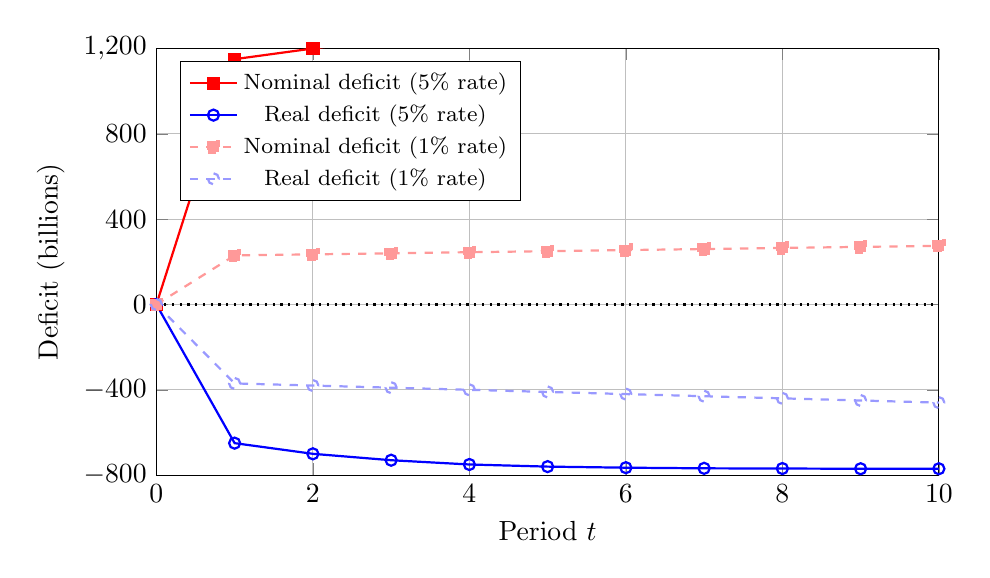
\begin{tikzpicture}
\begin{axis}[
    width=0.95\textwidth,
    height=7cm,
    xlabel={Period $t$},
    ylabel={Deficit (billions)},
    legend pos=north west,
    grid=major,
    xmin=0, xmax=10,
    ymin=-800, ymax=1200,
    xtick={0,2,4,6,8,10},
    ytick={-800,-400,0,400,800,1200},
    legend style={font=\footnotesize},
    every axis plot/.append style={thick}
]

% Nominal deficit - rate hike scenario (5% rate)
\addplot[color=red, mark=square*] coordinates {
    (0,0) (1,1150) (2,1200) (3,1250) (4,1300) (5,1350) (6,1400) (7,1450) (8,1500) (9,1550) (10,1600)
};
\addlegendentry{Nominal deficit (5\% rate)}

% Real deficit - rate hike scenario
\addplot[color=blue, mark=o] coordinates {
    (0,0) (1,-650) (2,-700) (3,-730) (4,-750) (5,-760) (6,-765) (7,-768) (8,-769) (9,-770) (10,-770)
};
\addlegendentry{Real deficit (5\% rate)}

% Nominal deficit - low rate scenario (1% rate)
\addplot[color=red!40, mark=square*, dashed] coordinates {
    (0,0) (1,230) (2,235) (3,240) (4,245) (5,250) (6,255) (7,260) (8,265) (9,270) (10,275)
};
\addlegendentry{Nominal deficit (1\% rate)}

% Real deficit - low rate scenario
\addplot[color=blue!40, mark=o, dashed] coordinates {
    (0,0) (1,-370) (2,-380) (3,-390) (4,-400) (5,-410) (6,-420) (7,-430) (8,-440) (9,-450) (10,-460)
};
\addlegendentry{Real deficit (1\% rate)}

\draw[dotted, thick] (axis cs:0,0) -- (axis cs:10,0);

\end{axis}
\end{tikzpicture}
\caption{Multi-period nominal vs.\ real deficit trajectories under high-debt scenario (120\% debt/GDP). Rate hike from 1\% to 5\% increases nominal deficit sharply (via interest payments) but produces \emph{larger real surplus} due to inflation erosion. Illustrates Mosler's deficit channel: rate hikes can be inflationary when debt is high.}
\label{fig:deficit-trajectories}
\end{figure}
